\chapter{Top-down Constraints on Atmospheric Mercury Emissions from ASGM Activities}
\section{Background}
\begin{flushleft}


 Numerous prior studies have quantified anthropogenic Hg sources, including ASGM Hg emissions using different methodologies. Bottom-up estimates leverage collected data on underlying activities and emission factors to estimate regional and global totals. For instance, the bottom-up global inventory in the GMA 2018 estimated ASGM Hg emissions to be 838 Mg with an uncertainty range of 675-1000 Mg for 2015 \cite{united_nations_environment_programme_technical_2019,steenhuisen_development_2019}. Moreover, Streets et al. (2019) tested six different proxies for scaling emissions to other years and used an average value to scale the inventory of emissions to the year 2015, thus estimating that ASGM was the largest source and responsible for 775 Mg of emissions\cite{streets_global_2019}. Muntean et al. (2014) also used a bottom-up technique in which they found that poverty in gold ore-rich countries (as measured by the GINI index \cite{sadefo_kamdem_nice_2012}, where available) was correlated with data on ASGM production activity. The poverty-based approach they used estimated that ASGM was responsible for 728.27 Mg emissions in 2010, equivalent to 41.1\% of the global Hg emissions\cite{muntean_evaluating_2018}. Such inventories are essential and a critical input to model Hg using CTMs such as \gc. However, the different assumptions on the activity data and emission factors induce significant uncertainty in the emission inventories. An additional bias in the bottom-up approach originates from the reliance on officially reported emissions data, which might cause differences in accuracy between countries and regions. 
 \end{flushleft}
 \begin{flushleft}
    National baseline Hg use estimates are bottom-up inventories where countries identify and quantify the sources of Hg released within their borders. Under Article 7 of the MC and Annex C, countries must include in their NAPs baseline estimates of the quantities of mercury used in ASGM within their territory \cite{united_nations_environment_programme_estimating_2017}.  
 \end{flushleft}
 



\begin{flushleft}
On the contrary, top-down emission estimation approaches combine atmospheric transport and chemistry models with atmospheric concentration measurements to quantify emissions. Even though the atmospheric chemistry literature has various top-down method applications, no study explicitly constrains ASGM Hg emissions. For instance, Bousquet et al., 1999 applied top-down methods to infer surface fluxes of atmospheric CO\textsubscript{2} from observed concentrations\cite{bousquet_inverse_1999}. Furthermore, Kopacz et al., 2009, employed top-down techniques to quantify source contributions to ozone pollution at two adjacent sites on the U.S. west coast in the spring of 2006. They highlight that they used  \gc as a common intercomparison platform to show global consistency between the different satellite datasets and the in situ data. This underscores the role models such as GEOS-chem have as integration platforms for differently sourced data to generate unified insights. Likewise, Hg emissions have been constrained using top-down methods in Song et al., 2015 where a top-down approach at a global scale is applied to quantitatively estimate present-day Hg emission sources and critical parameters in GEOS-Chem to better constrain the global biogeochemical cycle of Hg. Moreover, Denzler et al., 2017 used a top-down approach to quantify Hg emissions on a European scale based on the atmospheric Hg measurements conducted at the remote high-altitude monitoring station, Jungfraujoch, Switzerland. 
\end{flushleft}
\begin{flushleft}
In this chapter, I apply a top-down approach at a regional scale to estimate ASGM Hg emissions (emission inversion) from Peru. Until now, no scientific studies have provided top-down constraints for ASGM emissions using atmospheric transport models and Hg atmospheric monitoring data. Section 3.2 describes the overall methodology. I combine ground-based observations of atmospheric Hg from the case study region\cite{koenig_seasonal_2021}, a national inventory for Peru\cite{artisanal_gold_council_reporte_2017} and simulations with the GEOS-Chem global CTM. Reference (also known as a priori) emissions are from the GMA 2018\cite{steenhuisen_development_2019,united_nations_environment_programme_technical_2019}. The Markov Chain Monte Carlo is the inversion method used (Sect. 3.2.2) to obtain the optimized (a posteriori) emissions, considering uncertainties associated with reference and ground-based observations. Section 3.3 presents results and discussion. Comparisons of observations and model outputs are given in Sect. 3.3.1. The optimized emissions from 5 regions in Peru are shown in Sect. 3.3.2 Finally, I discuss the implications of the inversion results for providing baseline estimates of ASGM Hg emissions  and summarize my conclusions (Sect. 3.3.4).

\end{flushleft}
\newpage
\section{Methods}
\begin{flushleft}
    In the results section of chapter two of this thesis, I discussed the differences between the \gc model predictions of Hg at various measuring stations and in Latin America. One of the hypotheses proposed attributed the differences between the model and the observations to how the emissions were parameterized in \gc. The input emissions in \gc are determined by the Hg inventory; hence, I first evaluated the Hg inventory used in the model against other global inventories. Next, the inventory was compared to a national inventory for Peru \cite{agc_reporte_2017}. Once the differences between the global inventory\cite{steenhuisen_development_2019} and the Peruvian national inventory were analyzed, the global inventory was re-gridded to the GEOS-Chem grid, and the emissions from grid boxes corresponding to different departments in Peru were scaled. The scaled inventories were used to create the simulations described in Table \ref{tab:all_geos_chem_simulations}. These simulations were used to determine the sensitivity of the Hg concentration at distant locations to the changes in emissions from the grid boxes in the case study region. The simulated \hgc in the atmosphere was compared to the observed TGM concentration in the atmosphere to determine the sensitivity of the \hgc to the changes in emissions from individual grid boxes and multiple grid boxes. 
\end{flushleft}

\subsection{Mercury Emission Inventories}
\begin{flushleft}


Globally gridded emissions inventories such as those shown in Figure \ref{fig:Hg_inventories} are a critical input to CTMs such as \gc. The GMA 2018 ASGM emissions estimates for the year 2015 were used in all the GEOS-Chem simulations we carried out. This inventory was used because it was more representative of the ASGM emissions than the other two inventories. ASGM emissions in this inventory were distributed based on a system that uses a probability approach to estimate ASGM activity and then distributes the emission estimate according to that probability\cite{steenhuisen_development_2019}. The global alluvial gold map for  and a (gold) mining concessions  \href{(https://data.globalforestwatch.org/search?collection=Dataset&q=mining)}{data set} were used to distribute ASGM emissions for Peru. 
\end{flushleft}
\begin{figure}[H]
  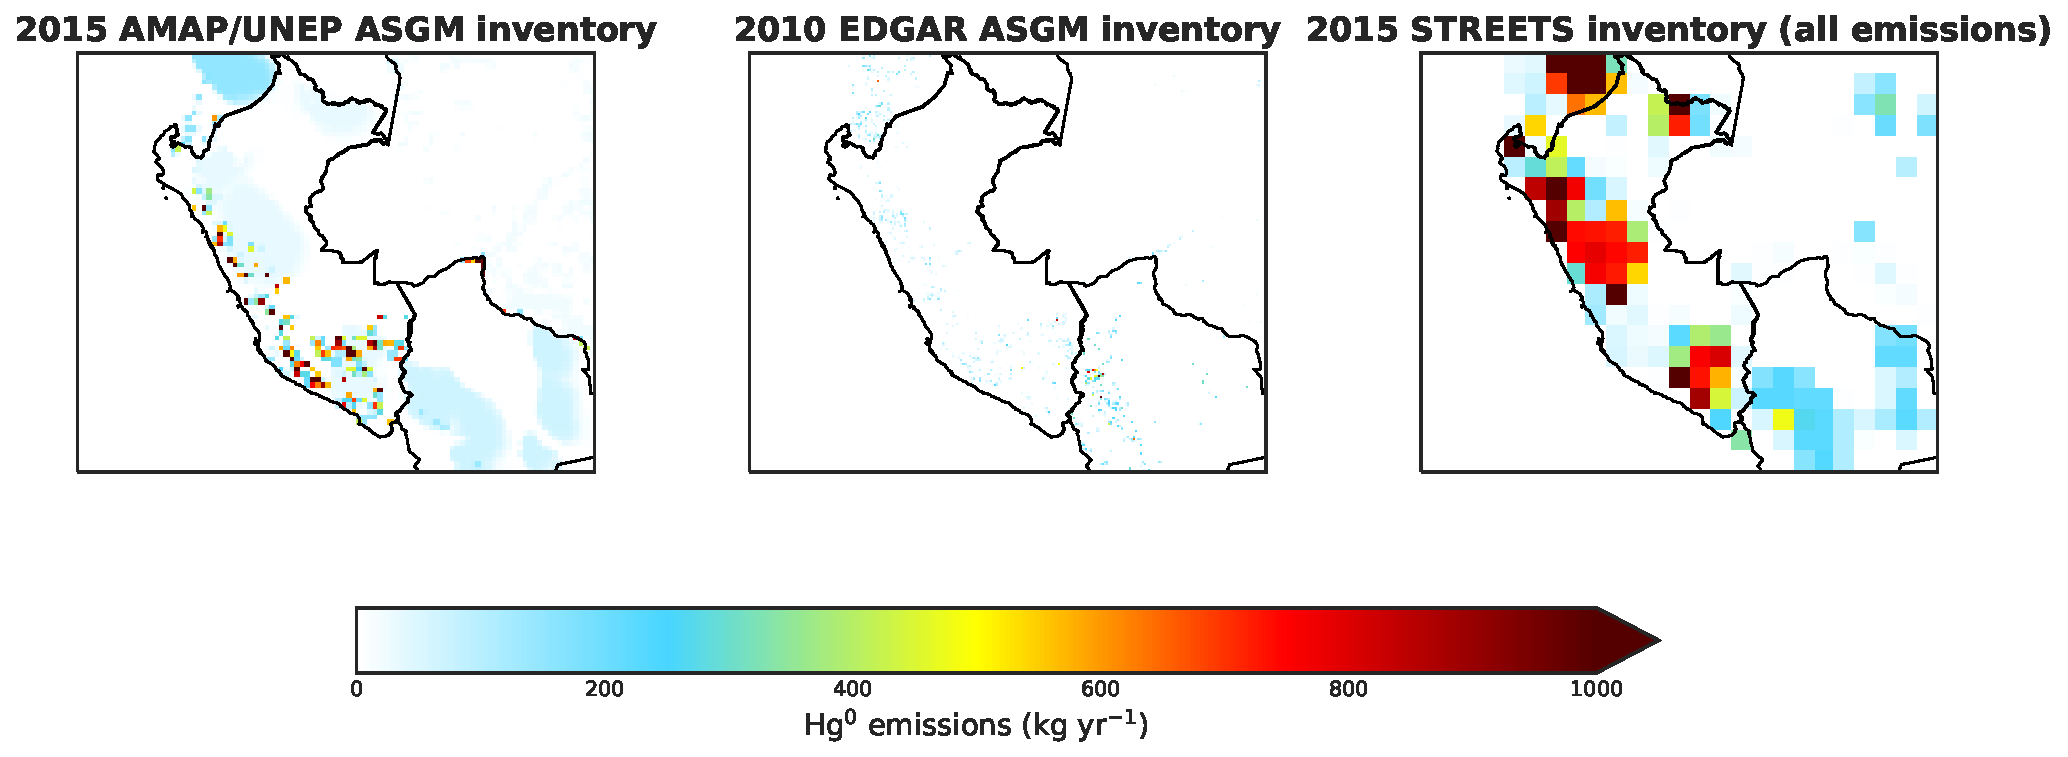
\includegraphics[width=\textwidth]{templates/figures/Peru_Maps/Hg_inventories.pdf}
  \centering
  \caption{Comparison of Hg emission from Peru as estimated by different global inventories \cite{united_nations_environment_programme_technical_2019,steenhuisen_development_2019,muntean_evaluating_2018,streets_global_2019}}
  \label{fig:Hg_inventories}
\end{figure}
\FloatBarrier


\subsection{Emission Modification and \gc Simulations}
\begin{flushleft}
    Six more simulations were added to the \on and \off \gc simulations presented in Chapter 2. The first additional simulation was similar to the \on but was  conducted at a higher resolution. The other five simulations were sensitivity runs that used modified emission inventories corresponding to changes in emissions from one of the grid boxes in the case study region.
\begin{figure}[H]
\centering

\begin{tabular}[H]{c}

\subfloat[GMA 2015 Grid]{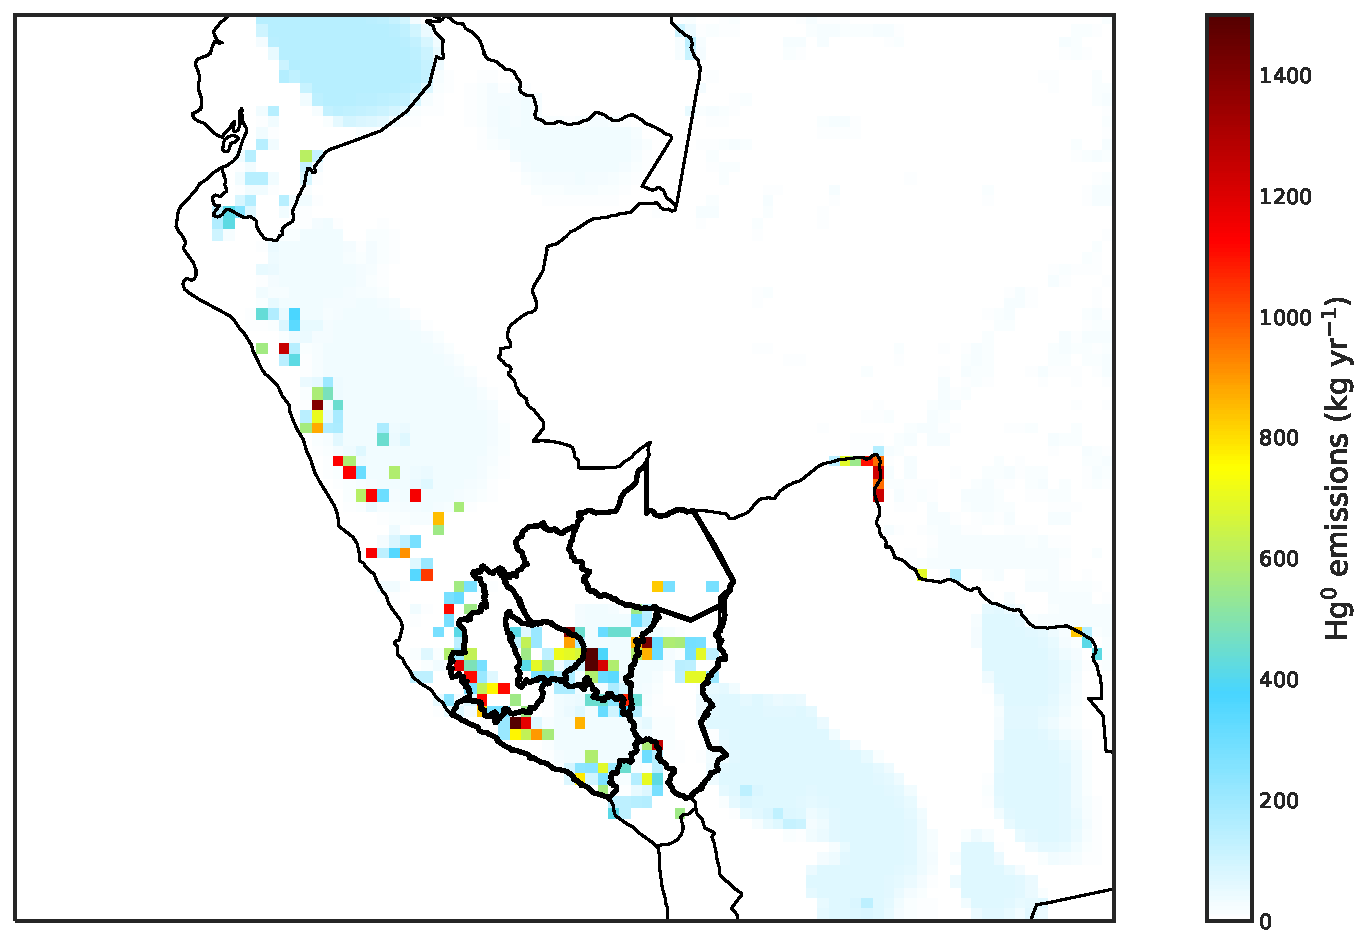
\includegraphics[width = 0.8\linewidth]{templates/figures/Peru_Maps/GMA2018inventory025x025.pdf}}\\
\subfloat[GEOS Chem Grid]{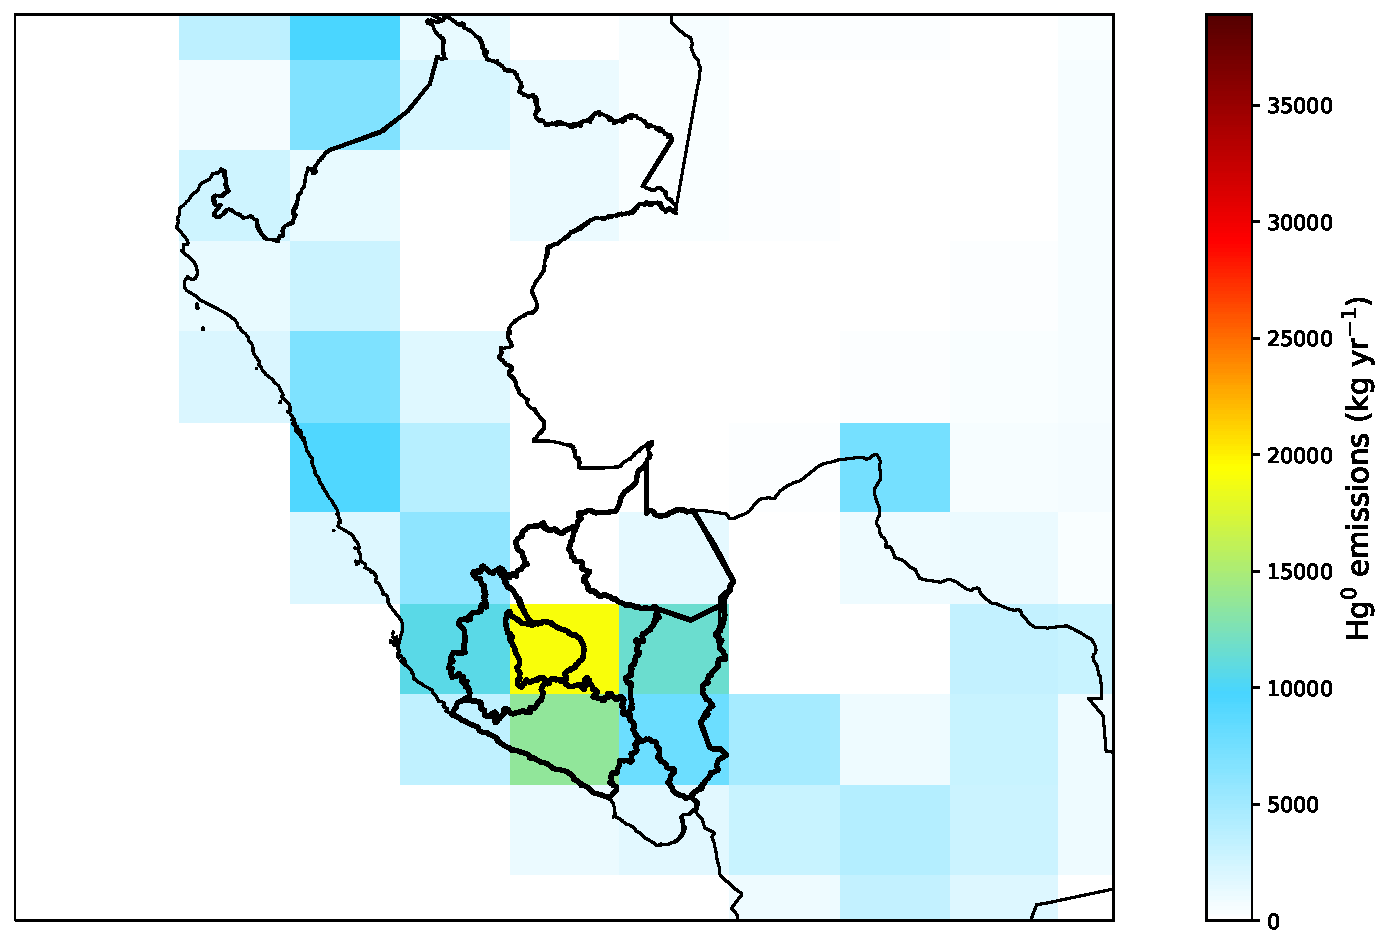
\includegraphics[width = 0.8\linewidth]{templates/figures/Peru_Maps/GMA2018inventory2x25.pdf}}


\end{tabular}
  

\captionof{figure}{Maps showing how the GMA2018 emission estimates for the year 2015 were distributed for Peru before re-griding (a) and after re-gridding to the \gc grid (b) }
\label{fig:GMA2018}
\end{figure}
\FloatBarrier
\end{flushleft}


\begin{table}[H]
\caption{Table showing the different GEOS-Chem simulations used in the analysis}
    \label{tab:all_geos_chem_simulations}
\begin{tabular}{lcp{0.5\linewidth}}

\textbf{Simulation Name}    &  Resolution       & \textbf{Description Estimate}                             \\
\hline
Base (ASGM=ON)              & 2.0$\times$2.5        & All Hg anthropogenic emission sources are turned on  \\
No ASGM (ASGM=OFF)          & 2.0$\times$2.5        & All ASGM emissions are turned off                     \\
Mdd                         & 2.0$\times$2.5        & Emissions from the \gc grid box located in  Madre de Dios  were scaled up by a factor of 2 \\

Apr                         & 2.0$\times$2.5        & Emissions from the \gc grid box located in Apurimac were scaled down by a factor of 0.5\\

Aqp                         & 2.0$\times$2.5        & Emissions from the \gc grid box located in Arequipa department were scaled up by a factor of 2\\

Npun                        & 2.0$\times$2.5        & Emissions from the \gc grid box located in the northern region of Puno were scaled up by a factor of 2 \\

Spun                        & 2.0$\times$2.5        & Emissions from the \gc grid box located in the southern region of the Puno were scaled up by a factor of 2 \\
\hline
\end{tabular}
\centering
\end{table}

\newpage
\subsection{Simulated Atmospheric Mercury Concentration Signals}
\begin{flushleft}
The relationship between the \hg emissions from a specific grid box and the \gc simulated atmospheric \hg concentration at distant points from the emissions source is assumed to be defined by a linear function. This means that an increase in emissions is expected to result in an increase in the \hg concentration. Consequently, the relationship between emissions and concentrations can be represented by the following equation:


\begin{equation}
\label{doublingSig}
Hg^0_{sig(region)}=Hg_{m_0}+\small\frac{(Hg_{m_1} -Hg_{m_0})}{(m_1 -m_0)}(m_{(region)} -m_0)
\end{equation}
where:
\end{flushleft}

\begin{description}[leftmargin=!,labelwidth={5 em}]
    \item [$region$] is the location of the emission source within the case study region.
    \item [$Hg^0_{sig(region)}$] is the simulated \hg concentration at the observation site due to $m_{(region)}$ at the grid box in the specific $region $ of interest.
    \item [$Hg_{m_0}$] is the Hg concentration  at the observation site generated by the Base (ASGM =ON) simulation. 
    \item [$Hg_{m_1}$] is the Hg concentration  at the observation site generated by the $i^{th}$ region simulation $i$=Mdd,Apr,Aqp,Npun,Spun. 
    \item [$m_1$] is the amount of emissions in Mega grams after scaling the emissions from a specific grid box.
    \item [$m_0$] is the amount of emissions in Mega grams before scaling the emissions from a specific grid box.
\end{description}


% \begin{flushleft}
% $Hg_{sig(region)}$ gives the Hg concentration signal in the atmosphere that results from a unit change in the tonnes of emissions from a specific grid box. Therefore, $Hg_{sig(region)}$ was used to investigate the sensitivity of the observations to the different amounts of additional ASGM Hg emissions and the regional grid boxes. The Hg concentration in the atmosphere that results from a specific change in emissions from a particular grid box was calculated using Equation \ref{ysignal} below.
% \begin{equation}
% \label{ysignal}
% \small{Hg_{m(region)}} =Hg_{sig(region)}(m-m_o), 
% \end{equation}
% where:
% \end{flushleft}


% \begin{description}[leftmargin=!,labelwidth={1.5 em}]
    
%     \item [$m_0$] is the GMA 2018 ASGM emissions estimate in metric tonnes for the particular grid box corresponding to a place in the case study region
    
%     \item [$m$] is the amount of emissions, in metric tonnes, from a grid box required to produce $Hg_{m}$ concentration in the atmosphere
% \end{description}




% \begin{flushleft}
% For each grid box in the case study region, the emissions were modified from their original GMA 2018 estimates to new values based on Hg emission estimates produced by the Artisanal Gold Council(AGC)
% \end{flushleft}

\subsection{Observation Site Selection}

\begin{flushleft}
TGM and GEM observation data from different locations in Latin America were analyzed and compared to the \gc simulated \hg concentrations for those sites in Chapter 2. The \gc predictions for ASGM contributions to atmospheric Hg concentration were higher at the CHC, making it an excellent candidate to use as a reference for comparison with the modified \gc Hg concentration predictions. Moreover, this site is the closest monitoring site to Peru hence it is expected that it would be more likely to detect atmospheric \hg changes that result from the changes in Hg emissions from the case study region. The time series of the observed concentration at the CHC station between July 2014 and January 2016 is shown in Figure\ref{fig:chc_time_series}.
\end{flushleft}

\begin{figure}[H]
  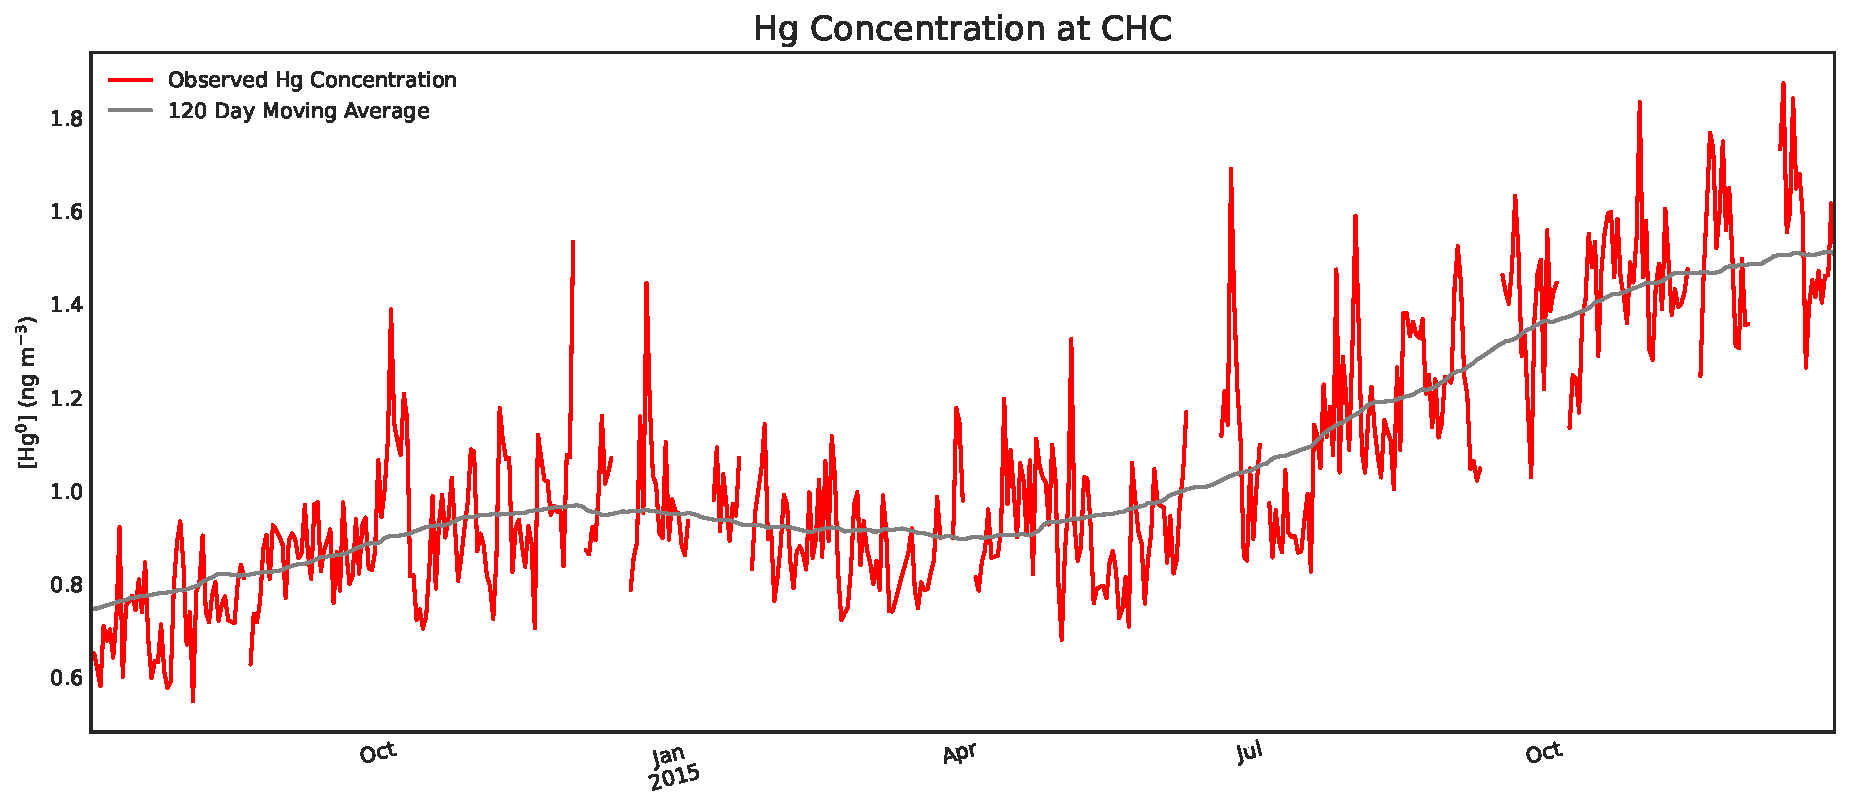
\includegraphics[width=\textwidth]{templates/figures/GMOS_Sites/ObsTimeSeries.pdf}
 
  \caption{The average daily TGM concentration at CHC in ngm\textsuperscript{-3} as a function of time over the measurement period from July 2014 to January 2016. The daily average concentration is indicated by the red line, while the grey line shows the 120-day moving average, which highlights the upward trend in the daily averages}
  \label{fig:chc_time_series}
  \centering
\end{figure}
\FloatBarrier
\begin{flushleft}

The detailed characteristics of the observations over this measurement period were described in Koening et al. (2020); hence our analysis focused on using the observation TGM data to evaluate the performance of the GEOS-Chem model in predicting the \hg based on the input \hg emission inventories. As shown in Figure \ref{fig:chc_time_series}, the TGM concentration at CHC showed an upward trend, which Koening et al. (2021) attribute to El Nio-Southern Oscillation\cite{koenig_seasonal_2021}. As a result, they categorized the measured TGM concentrations in the atmosphere at the CHC site as normal conditions (NC), 2013-07 to 2015-05, and ENSO conditions 2015-06 to 2016-01. To reduce the number of records associated with ENSO, I limited my analysis to one year's worth of data from 2014-07 to 2015-07.
\end{flushleft}

\subsection{Markov Chain Monte Carlo}

\begin{flushleft}
The Markov-Chain Monte Carlo (MCMC) is a sampling method that is also useful for fitting models to data\cite{hogg_data_2018}. We apply the MCMC to constrain ASGM Hg emissions from the case study region in Peru.  The model is generated by a set of parameters and emissions, and we aim to sample from the parameters that best fit our data. The MCMC is used to compare the modeled concentrations to the observed data using metrics such as the $95^{th}$ confidence interval, mean, and the interquartile range. The MCMC generatively models given data by sampling around optimum values from the posterior distribution. The MCMC is a Bayesian approach; hence it requires the definition of priors on the parameters of interest. The priors encode information that we already know of the system. The probability of the model given the observed data is given by the posterior probability, $P(\theta|D)$, which is calculated using the Bayes theorem:

\begin{equation}
\label{bayes_eq}
P(\theta|D)=\frac{P(D|\theta)P(\theta)}{P(D)}
\end{equation}
where:
\end{flushleft}

\begin{description}[leftmargin=!,labelwidth={3 em}]
    \item [$P(D|\theta)$] is the likelihood which is the probability of the data given the model
    \item [$P(\theta)$] is the prior, which is the probability of the model and 
    \item [$P(D)$] is the evidence which is the probability of the data.
\end{description}

\begin{flushleft}
The MCMC enables the estimation of the sampling of the posterior distribution, which is the left-hand side of Equation~\ref{bayes_eq}. The MCMC is set up by following a set of steps that include defining a function that outputs a model given a set of input parameters and establishing an ensemble of walkers defined by a $\theta$ vector that contains a set of parameters from the model generating function. For the model generating function, the Hg concentration at a particular grid box is defined as a linear combination of Hg concentration signals from the case study region and the baseline Hg concentration produced by the \on as shown in the Equation \ref{Hg_conc} below:

\begin{align}
\begin{split}\label{Hg_conc}
Hg_{conc}= {}&Hg_{m(MdD)}+ Hg_{m(S-Puno)} + Hg_{m(N-Puno)} + Hg_{m(Apr)}+ Hg_{m(Aqp)}\\
            & +Hg_{m_0}
\end{split}
\end{align}

where:
\end{flushleft}

\begin{description}[leftmargin=!,labelwidth={5 em}]
    \item [$Hg_{m(MdD)}$] is the Hg concentration signal resulting from emissions from the Madre de Dios (MdD) grid box
    \item [$Hg_{m(S-Puno)}$] is the Hg concentration signal resulting from emissions from the South Puno (S-Puno) grid box
    \item [$Hg_{m(N-Puno)}$] is the Hg concentration signal resulting from emissions from the North Puno (N-Puno) grid box
    \item [$Hg_{m(Apr)}$] is the Hg concentration signal resulting from emissions from the Apurimac (Apr) grid box
    \item [$Hg_{m(Aqp)}$] is the Hg concentration signal resulting from emissions from the Arequipa (Aqp) grid box
    \item [$Hg_{m_0}$] is the baseline Hg concentration signal.
\end{description}

\begin{flushleft}
Each of the $Hg_{m(region)}$ terms of Equation \ref{Hg_conc} represent signals from the different departments are calculated using Equation~\ref{doublingSig}. The $m_(region)$ terms are the only unknowns and the equation can be expanded to isolate the terms with $m_(region)$, which is the parameter we are optimizing for in the MCMC method. The expanded form of Equation \ref{Hg_conc} is shown below:

\begin{align}
\begin{split}\label{Cs36PoGd2l}
Hg_{conc}={}& (m_{(MdD)}Hg_{sig_{(MdD)}} -m_oHg_{sig_{(MdD)}})+ (m_{(S-Puno)}Hg_{sig_{(S-Puno)}} -m_oHg_{sig_{(S-Puno)}}) \\
            &+ (m_{(N-Puno)}Hg_{sig_{(N-Puno)}} -m_0Hg_{sig_{(N-Puno)}}) + (m_{(Apr)}Hg_{sig_{(Apr)}} -m_oHg_{sig_{(Apr)}}) \\
            &+ (m_{(Aqp)}Hg_{sig_{(Aqp)}} -m_oHg_{sig_{(Aqp)}})+Hg_{m_0}
\end{split}
\end{align}

Since the values of $m_{(region)}$ are the parameters that we want to estimate using MCMC, they can be represented as $\theta_i=m_{(region)}, i=1$ and the other terms, including the background concentration, are combined into one constant, C:

\begin{equation}
\begin{aligned}
    Hg_{conc}  & = \theta_0C  + \theta_1Hg_{sig_{(MdD)}}+ \theta_2Hg_{sig_{(S-Puno)}} +  \theta_3Hg_{sig_{(N-Puno)}} \\
                & \ \ \ \  +\theta_4Hg_{sig_{(Apr)}} +  \theta_5Hg_{sig_{(Aqp)}}
\end{aligned}
\end{equation}

\begin{align}
Hg_{conc} =\begin{bmatrix} C & Hg_{sig_{(MdD)}} & Hg_{sig_{(S-Puno)}} &Hg_{sig_{(N-Puno)}} &Hg_{sig_{(Apr)}} &Hg_{sig_{(Aqp)}}\end{bmatrix} \times 
            \begin{bmatrix} \theta_0 \\ \theta_1 \\ \theta_2\\ \theta_3\\ \theta_4\\ \theta_5  \end{bmatrix}
\end{align}
where $\theta_0=1$ and $Hg_{conc}$ is the modeled Hg concentration at the observation site of interest.
\end{flushleft}

\begin{flushleft}
Next, the metrics being compared to their observed counterparts are calculated to be used in Equation \ref{model_definition} during the MCMC simulation. 
\end{flushleft}

% \begin{align}
% \begin{split}\label{model_definition}
% \hat{y}= {}&Hg_{m(MdD)}+ 
% \end{split}
% \end{align}


\newpage
\section{Results and Discussion}
\subsection{GEOS-Chem Predictions vs. Observations at Chalcataya}

\begin{figure}[H]
\centering

\begin{tabular}[H]{cc}

\subfloat[GMA 2015 Grid]{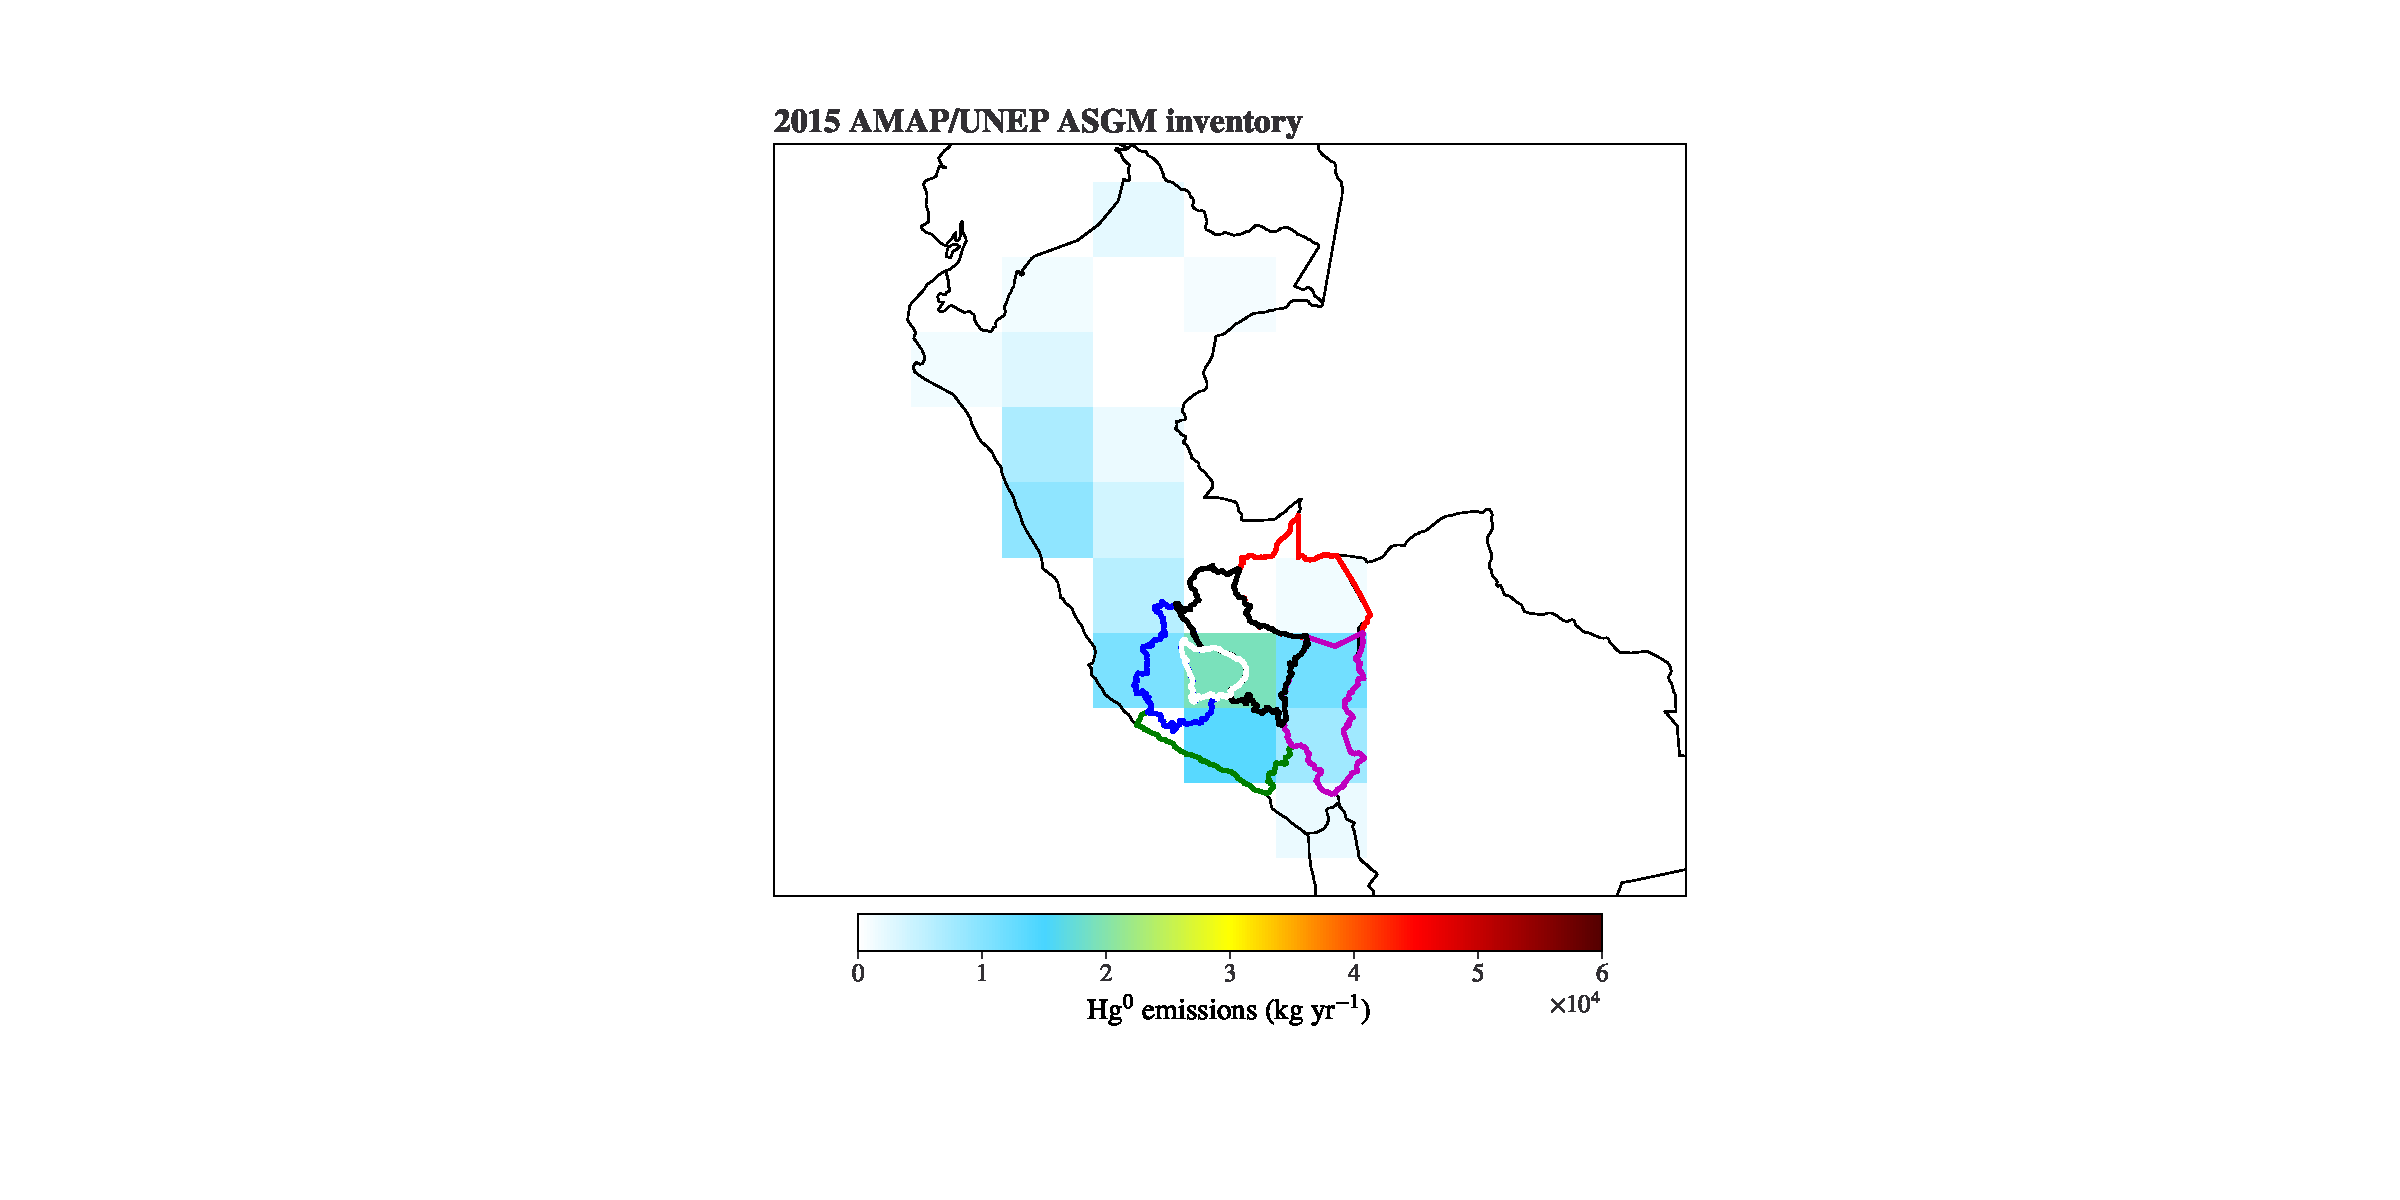
\includegraphics[width = 0.45\linewidth]{templates/figures/Peru_Maps/GMA2018inventory2x25Peru.pdf}}
\subfloat[GEOS Chem Grid]{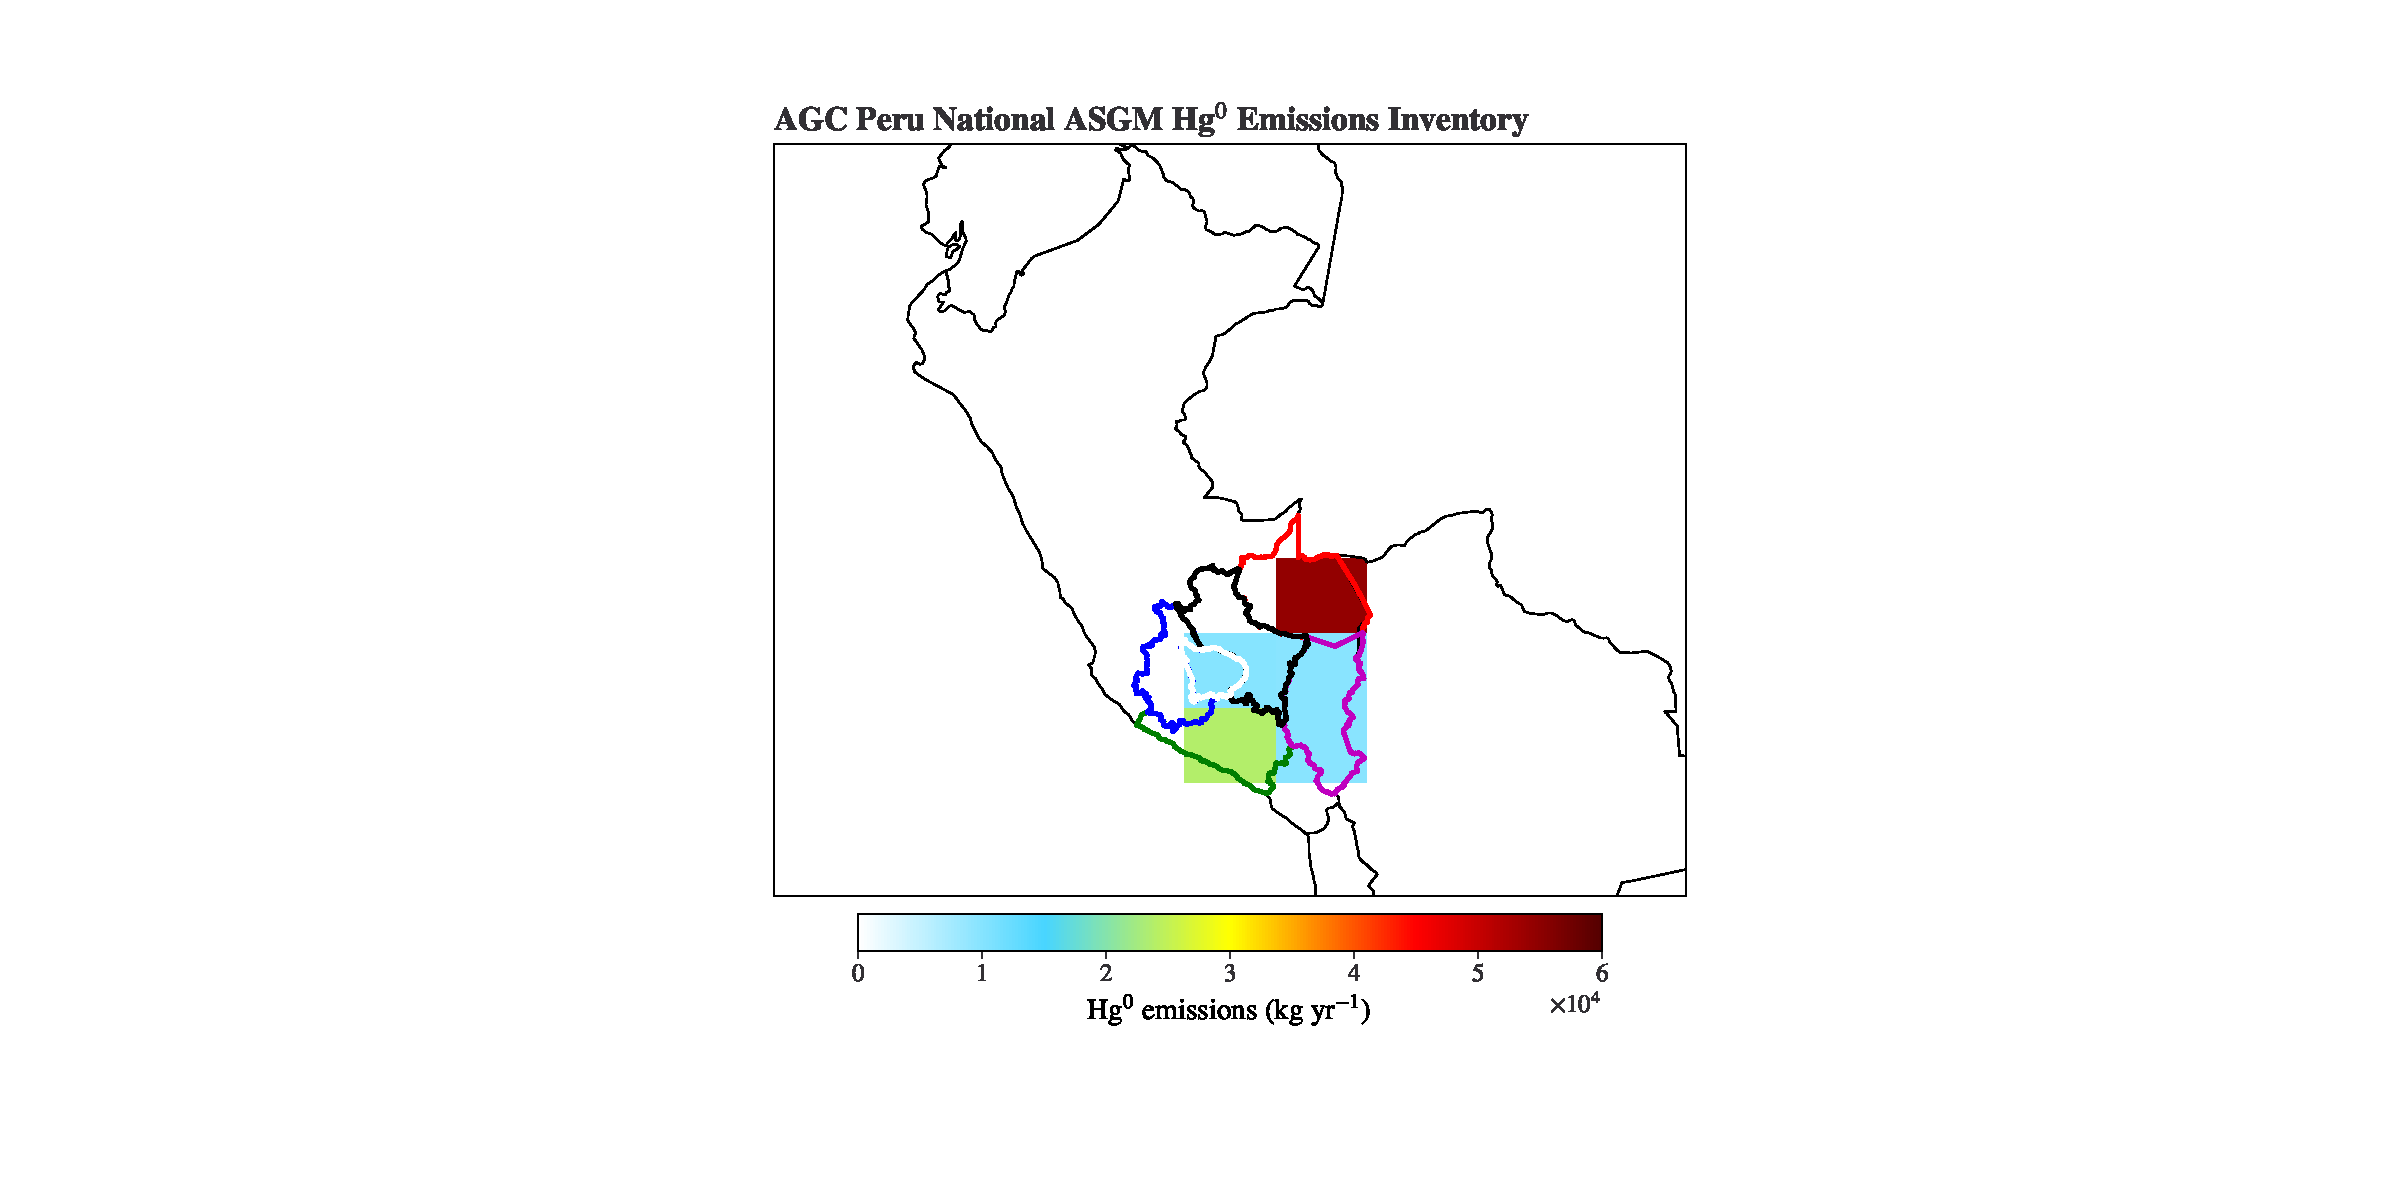
\includegraphics[width = 0.45\linewidth]{templates/figures/Peru_Maps/AGCinventory2x25Peru.pdf}}\\


\end{tabular}
  

\captionof{figure}{Maps showing how the GMA2018 emission estimates for the year 2015 were distributed for Peru before re-griding (a) and after re-gridding to the \gc grid (b) }
\label{fig:GMA2018}
\end{figure}
\FloatBarrier


\begin{flushleft}
The summary statistics of the \gc predicted \hgc at CHC for the one-year period from 2014/07/03 to 2015/07/03 compared to the observed atmospheric TGM concentration at CHC during the same period are shown on Table \ref{tab:ModelvsObsStats}. The mean \hg concentration produced by the \off  was within 1\% of the observed TGM concentration as seen in Table \ref{tab:ModelvsObsStats}. On the contrary, the average \hg produced by the \on shown by the blue line plot on Figure \ref{fig:ModelvsObsNstats} overestimated the mean by 29\%.
\end{flushleft}
\setlength{\tabcolsep}{2.5pt}
\begin{table}[H]
  \begin{center}
    \caption{Characteristics of observed and modeled Hg concentration in CHC where $\mu$ is the annual average Hg concentration, $\sigma$ is the standard deviation, $iqr$ is the interquartile range, $r_s$ is the Spearman correlation, $r$ is the Pearson correlation }
    \label{tab:ModelvsObsStats}
    \begin{tabular}{lccccc}
       %<-- added & and content for each column
      
                            & $\mu$                 & $\sigma$              & $iqr$                 & & \\
                            &  (ng m$^{-3}$)/year)  & (ng m$^{-3}$)/year)   & (ng m$^{-3}$)/year)   & & \\
     \cmidrule{2-4}
     Observations           & 0.90                  & 0.16                  & 0.18                  &  & \\
     \textbf{Simulations}   &                       &                       &                       &\textbf{$r_s$} &\textbf{$r$} \\ %
      \hline
      No ASGM (ASGM=OFF)    & 0.91                  & 0.06                  & 0.11                  & 0.170          & 0.144        \\ 
      Base (ASGM=ON)        & 1.16                  & 0.14                  & 0.20                  & 0.124         & 0.101         \\ % <--
    \end{tabular}
  \end{center}
\end{table}
\FloatBarrier
\begin{flushleft}
   The simulated \hg  and the observed TGM concentration at CHC are compared in detail in Figure \ref{fig:ModelvsObsNstats}. The observations (in red) are plotted as a function of time in plots (a) and (c) with the \off (in green) in plot (a)  the \on in (blue) in plot (c). The scatter plots in (b) and (d) represent the modeled \hg  as a function of the measured TGM concentration. The scatter plot in (b) shows that the variability in the observed TGM concentration is not captured by the \off simulation, while the scatter plot in (d) shows that the \on overestimates the observed TGM concentration values even though it closely approximates the variability in the values. The visible variability on the plots confirms the values presented in Table \ref{tab:ModelvsObsStats} where the \off  has a 62.5 \% lower standard deviation than the observed TGM concentration while the \on simulation's standard deviation is only 12.5 \% lower than the observed standard deviation in the TGM concentration. 
\end{flushleft}

\begin{flushleft}
    Even though GEOS-Chem closely approximated the mean Hg concentrations at CHC in the \off, the Spearman ($r_s$) and Pearson ($r$) correlations between the modeled and observed concentrations were very low at 0.17 and 0.144, respectively. Moreover, the coefficient of determination, $R^2$ between the observed and modeled concentrations in \off the case was almost zero at 0.0207. Brasseur and Jacob (p.471 2017) argue that in cases where a model captures the observed means but not the observed variability, the mean may be wrongly interpreted \cite{brasseur_modeling_2017}. In the case of \off, the mean may be wrongly interpreted because of the exclusion of the ASGM Hg emissions or the poor parameterization of vegetation uptake of Hg in the model. 
\end{flushleft}

\begin{figure}[H]
  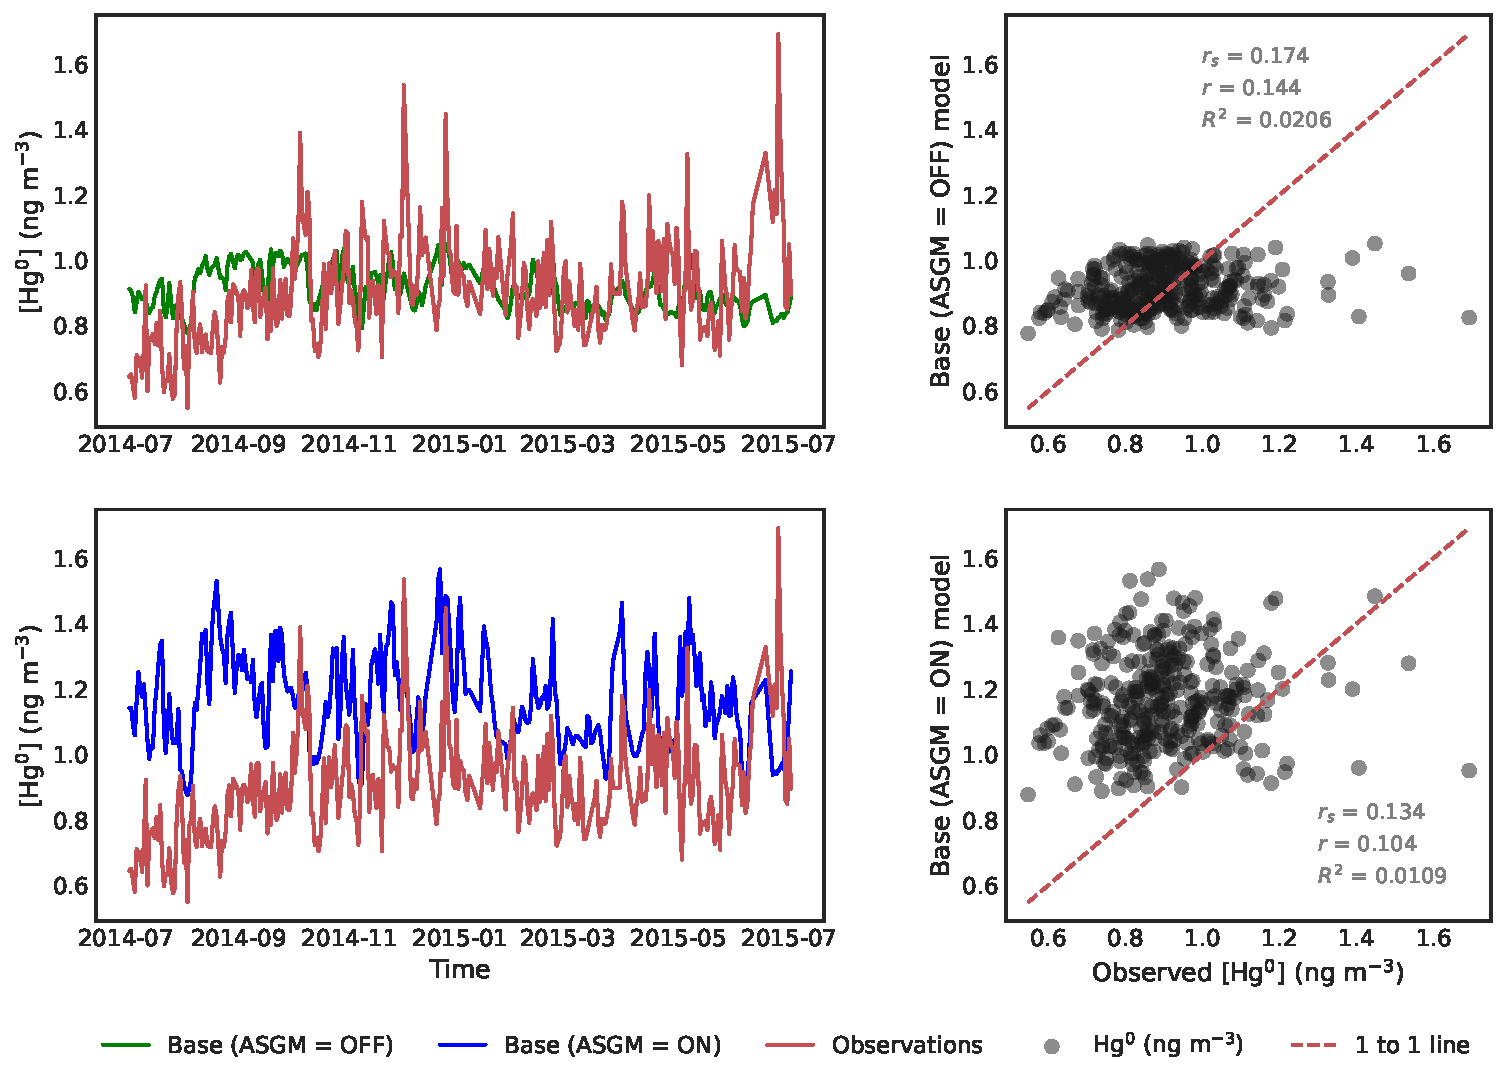
\includegraphics[width=0.85\textwidth]{templates/figures/ModelvsObs/TimeSeriesNsactter_obsVmodel_v1.pdf}
  \centering
  \caption{The observations (in red) are plotted as a function of time in plots (a) and (c) with the \off (in green) in plot (a) and the \on in (blue) in the plot (c). Analysis of the observed Hg concentrations vs. the \off  shows how the modeled mean closely approximates the observed mean and poorly estimates the daily variability, as shown by the difference in the size of the daily spikes of the Hg concentrations. The scatter plots in (b) and (d) represent the modeled \hg  as a function of the measured TGM concentration.}
  \label{fig:ModelvsObsNstats}
\end{figure}
\FloatBarrier

\begin{flushleft}
The relationship between the mean and variance in the observed and modeled  atmospheric Hg concentration at CHC was further explored as shown in Figure \ref{fig:Histplots} which shows the extent to which the GEOS-Chem model reproduces the mean and $iqr$ range of the observations. The \on  slightly overestimated (11\%) the $iqr$ of the Hg concentration in the atmosphere and overestimated the mean \hg by 29\%.  
\end{flushleft}

\begin{figure}[H]

\begin{tabular}[H]{cc}

\subfloat[]{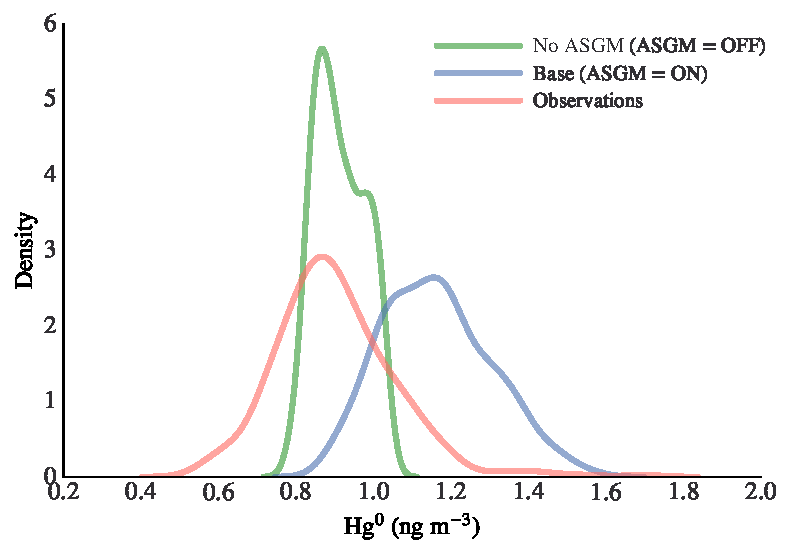
\includegraphics[width = 0.5\linewidth]{templates/figures/ModelvsObs/06-12-22_models_vs_observations_density-plot.pdf}} &
\subfloat[]{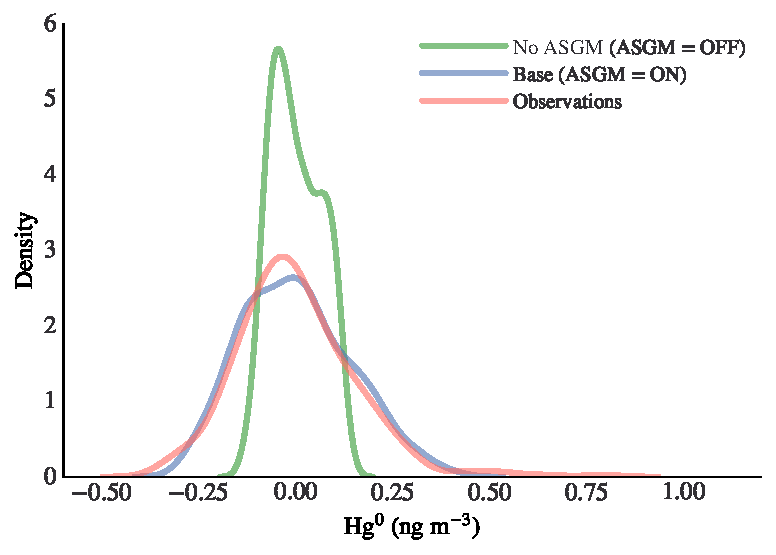
\includegraphics[width = 0.5\linewidth]{templates/figures/ModelvsObs/06-12-22_models_vs_observations_density-plot_std.pdf}}
\end{tabular}
\centering
\captionof{figure}{Density plots of the modeled and observed Hg concentration at Chalcataya. In (a), the actual distributions are plotted where the observed TGM concentration distribution is shown in red, the distribution of the \hgc predicted by the \off is shown in green, and that produced by the \on is shown in blue. In (b), the same distributions are shown after standardization by subtracting the mean in each distribution to see how the shapes of the distributions compare with each other.}
\label{fig:Histplots}
\end{figure}
\FloatBarrier

\begin{flushleft}
The poor reproduction of the observed average Hg concentration in the atmosphere by GEOS-Chem may be attributed to the model's poor parameterizations discussed in Chapter 2, such as the low vegetation uptake of Hg. 

\end{flushleft}
\newpage
\subsection{Comparison of Observations with Emission Modification}
The sensitivity of the modeled \hgc at the observation site to the changes in emissions from a single grid box in the case study region was investigated by finding the mean, IQR, and correlation as functions of the emissions from the specific grid box. The comparisons of how the modeled average \hgc at the observation site changes with an increase in emissions is shown in Figure \ref{fig:mean_vs_emissions}. As seen in the figure, the average modeled \hgc increases linearly with the increase in emissions for all of the sites.  Negative emissions represent a theoretical reduction in emissions.

\begin{figure}[H]
  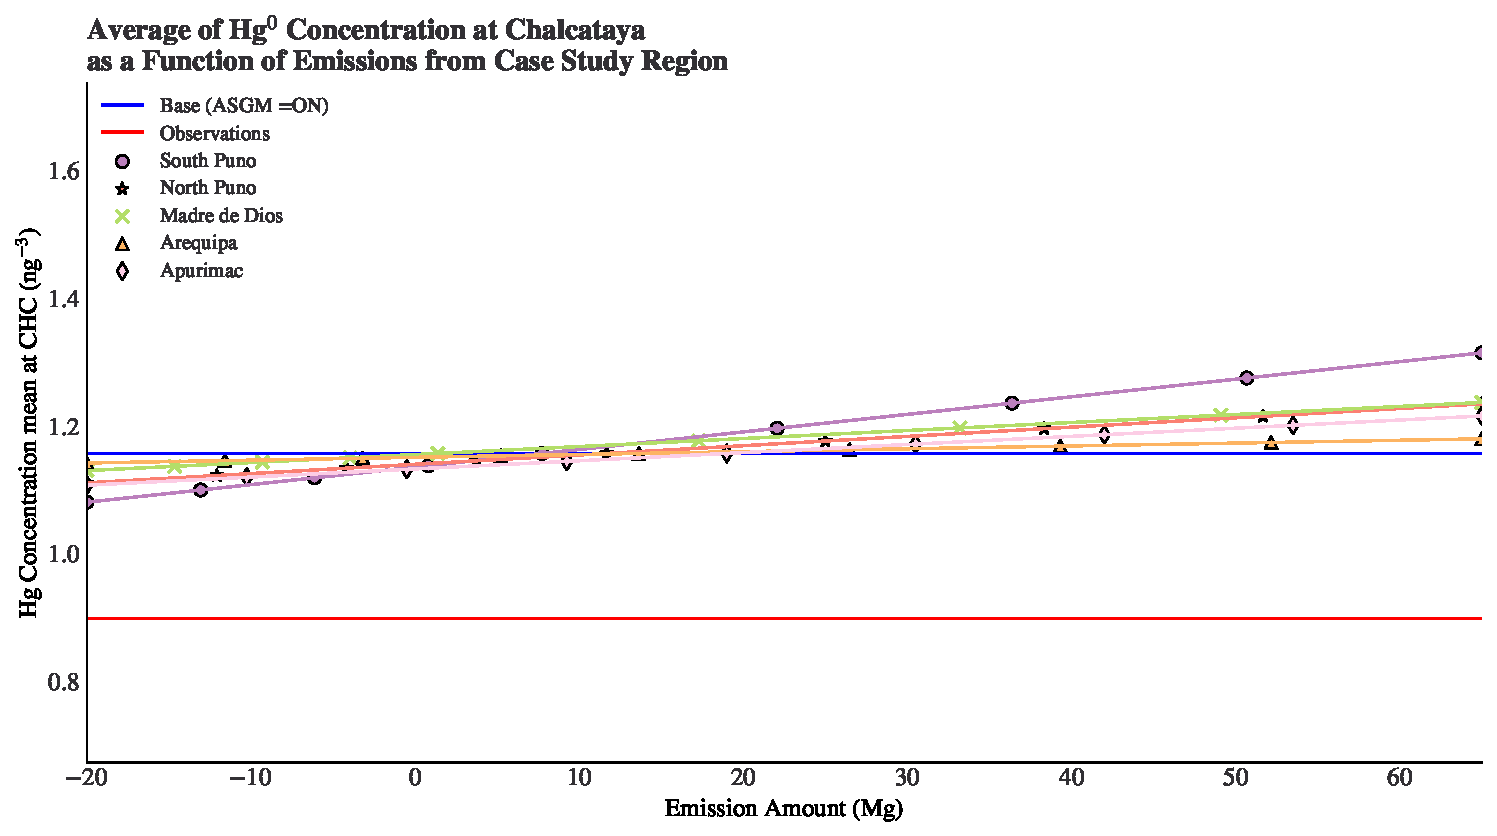
\includegraphics[width=\textwidth]{templates/figures/individual_site_modifications/mean_vs_emissions.pdf}
  \centering
  \caption{Modeled average atmospheric \hg concentrations at CHC over the period between 2014/07-2015/07. The red horizontal line indicates the y coordinate observed average TGM concentration of 0.90. The blue horizontal line indicates the average value of the \hg predicted by the \on. The following shapes show the relationships between the concentration at CHC and the emissions from grid boxes in the case study region: South Puno(circles), North Puno (stars), Madre de Dios (green cross), Arequipa (triangle), Apurimac (diamond)  }
  \label{fig:mean_vs_emissions}
\end{figure}
\FloatBarrier
\begin{flushleft}
    The rate of change of the \hgc with the increases in emissions ranges from X for emission increases at Arequipa to Y for emission increases in South Puno. Contrary to Figure \ref{fig:mean_vs_emissions} where the relationship between the number of emissions and the \hgc seems to be uniform, the relationship between the iqr and the emissions in Figure \ref{fig:iqr_vs_emissions}is not uniform across all of the sites.
\end{flushleft}

\begin{figure}[H]
  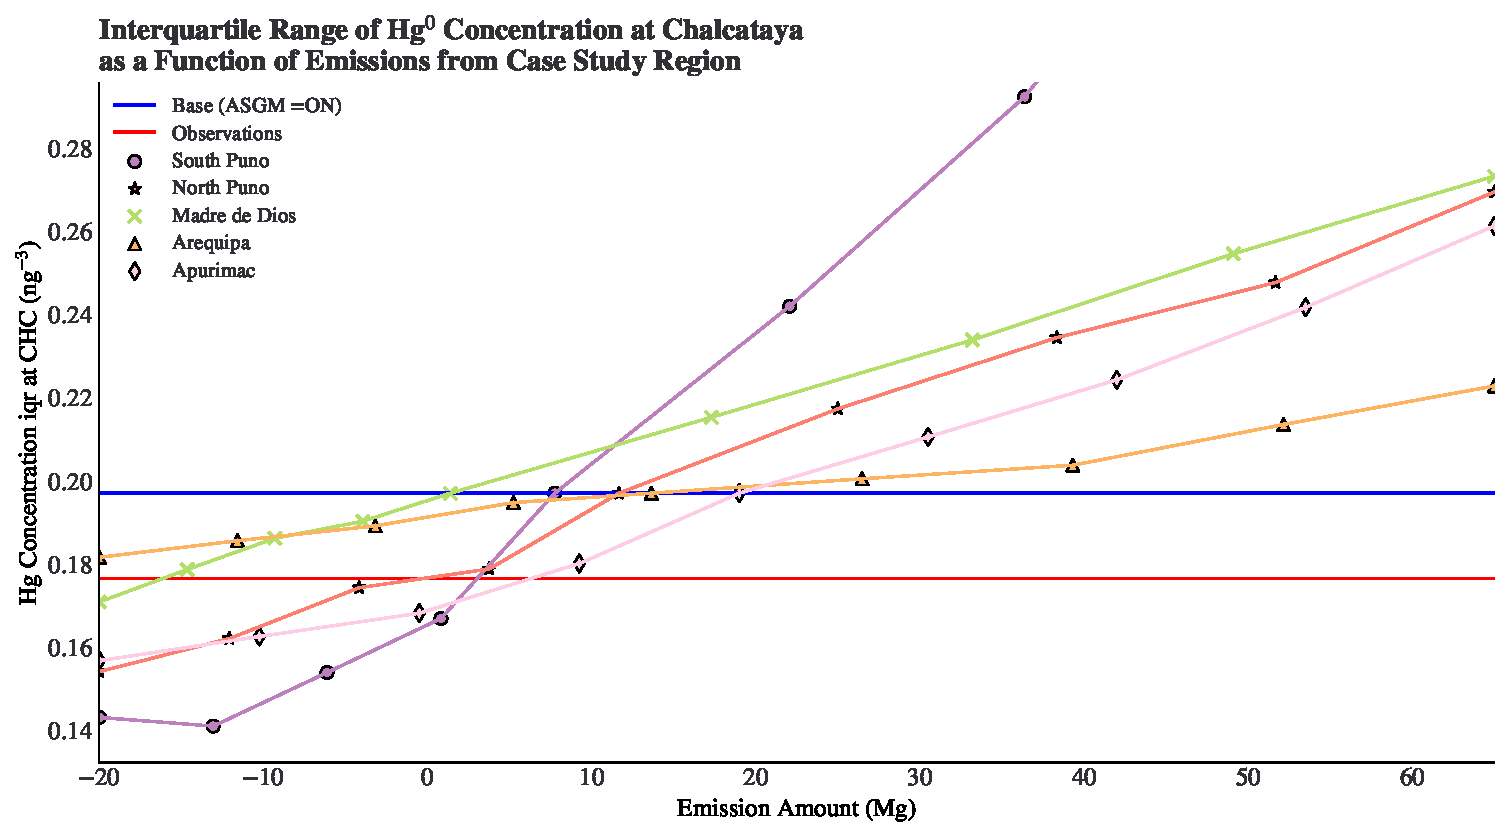
\includegraphics[width=\textwidth]{templates/figures/individual_site_modifications/iqr_vs_emissions.pdf}
  \centering
  \caption{ Observed and modeled atmospheric \hg concentrations IQR at CHC over the period between 2014/07-2015/07 as a function of emissions. The red horizontal line indicates the observed TGM concentration IQR(0.18). The blue horizontal line indicates the \on predicted \hg IQR. The following shapes show the relationships between the modeled \hg concentration signal IQR at CHC as a function of the emissions from grid boxes in the case study region: South Puno(circles), North Puno (stars), Madre de Dios (green cross), Arequipa (triangle), Apurimac (diamond)  }
  \label{fig:iqr_vs_emissions}
\end{figure}
\FloatBarrier
\begin{flushleft}
    The red and blue horizontal lines indicate the values of the observed Hg concentration and \on Hg concentration IQRs. The line represents how the IQR changes as emissions intersect the red line at least once, which means the observed IQR can be matched by changing emissions from one site. However, most lines intersect the red line when the emissions are negative, indicating that the emissions need to be reduced to match the observations. Reducing the emissions, especially emissions from the Madre de Dios region, is not a plausible course of action because bottom-up estimates show that the emissions from Madre de Dios are higher. Consequently, the fact that the lines on Figure \ref{fig:iqr_vs_emissions} intersect with the line representing the observed IQR cannot be interpreted to mean that the observed \hgc IQR can be approximated by increasing or reducing the emissions from a single source region. In contrast to the relationships evident in Figures \ref{fig:mean_vs_emissions} and \ref{fig:iqr_vs_emissions}, where the increase in emissions from all the sites leads to an increase in the \hgc, the relationship between the emissions and  correlation of the modeled \hgc and observed Hg concentrations  shown in Figure \ref{fig:correlation_vs_emissions}is negative for the South Puno, Arequipa, and Apurimac grid boxes. These relationships depicted in this Figure cement the fact that changing the emissions from one source in the\gc model does not improve the model's prediction of the observed concentrations. This section has attempted to show the effect of changing emissions from individual grid boxes on the modeled \hgc at a distant observation site. It is not surprising that emission modifications at one site did not improve \gcs \hgc because a comparison of bottom-up inventories such as the Peru national inventory of emissions developed by the Artisanal Gold Counsel\cite{agc_reporte_2017} and the global inventory in the GMA 2018\cite{steenhuisen_development_2019,united_nations_environment_programme_technical_2019} shows mismatches between the emissions estimates for multiple sites. 
\end{flushleft}

\begin{figure}[H]
  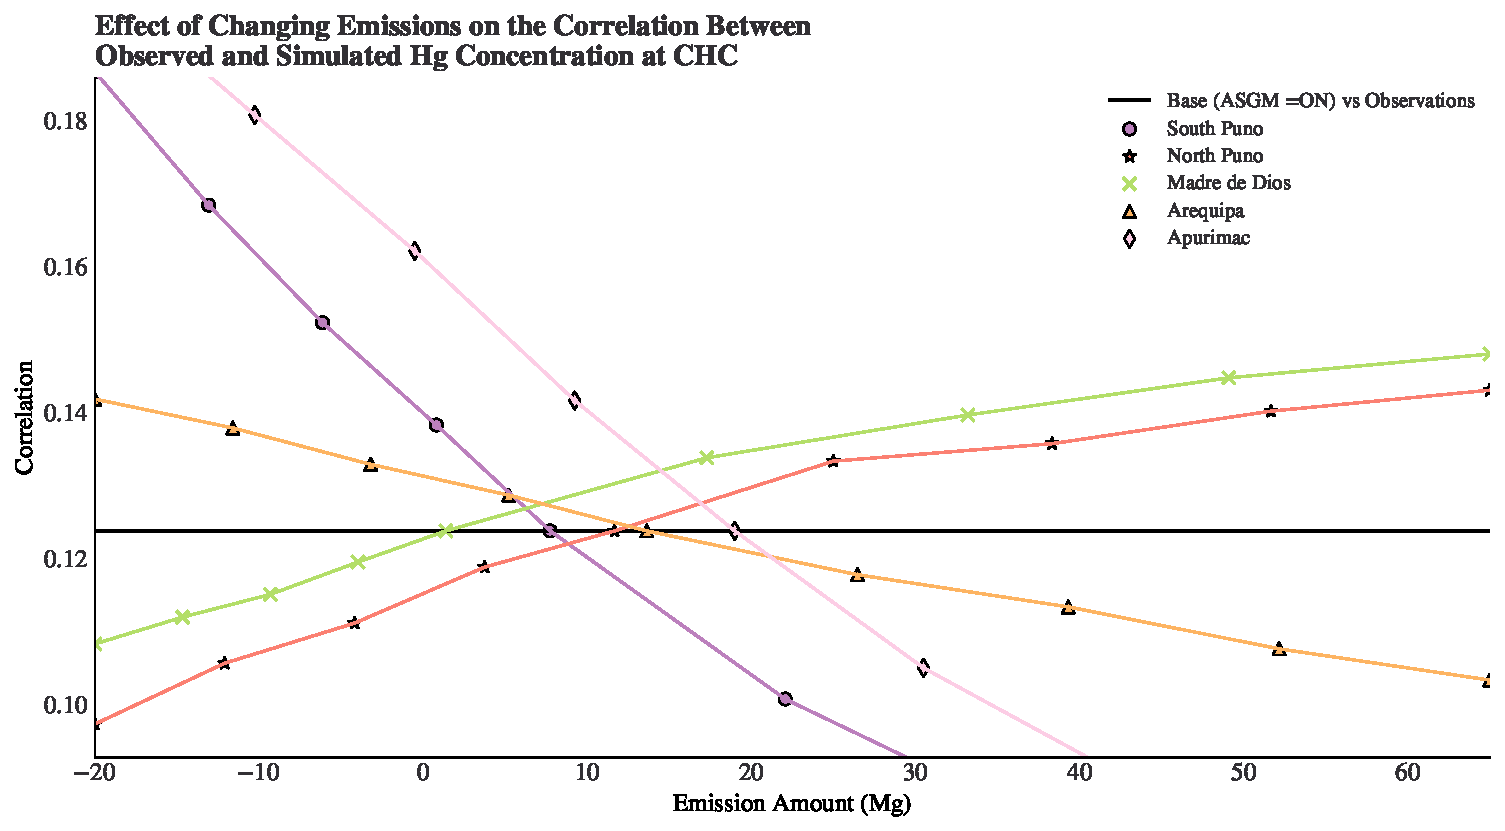
\includegraphics[width=\textwidth]{templates/figures/individual_site_modifications/correlation_vs_emissions.pdf}
  \centering
  \caption{Correlation between the observed and modeled atmospheric Hg concentrations at CHC over the period between 2014/07-2015/07 as a function of emissions from grid boxes associated with the case study region. The red horizontal line indicates the observed TGM concentration IQR(0.18). The blue horizontal line indicates the \on predicted \hg IQR. The following shapes show the relationships between the modeled \hg concentration signal IQR at CHC as a function of the emissions from grid boxes in the case study region: South Puno(circles), North Puno (stars), Madre de Dios (green cross), Arequipa (triangle), Apurimac (diamond)}
  \label{fig:correlation_vs_emissions}
\end{figure}
\FloatBarrier
\begin{flushleft}
   In the next section, I will present the principal findings of using the MCMC to investigate the effect of changing emissions from multiple sites instead of changing the emissions from one site as discussed in this section.
 
\end{flushleft}
\newpage
\subsection{Markov Chain Monte Carlo Simulation }
% \renewcommand{\arraystretch}{2}
\begin{figure}[H]
  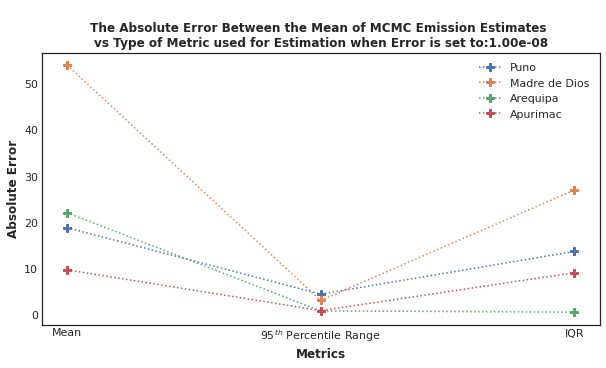
\includegraphics[width=\textwidth]{templates/figures/MCMC/comparison of matrics.png}
  \centering
  \caption{Comparison of the absolute error of different metrics when used in the MCMC to generate estimates of the emissions from different grid boxes in the case study region. The Absolute error is presented as a function of the type of metric used. The plus signs show the absolute error in reproducing emissions from the case study region(Puno (blue), Madre de Dios (orange), Arequipa (green), and Apurimac (red)) for each metric.  }
  \label{fig:MCMC_emetrics}
\end{figure}
\FloatBarrier
\begin{flushleft}
   As seen in Figure \ref{fig:MCMC_emetrics}, the 95$^{th}$ percentile range reproduce the GMA emissions estimates with the least absolute error, followed by the IQR. The mean was the worst metric to use in the MCMC to reproduce the emission estimates. This further corroborated the earlier finding that the mean was not a reliable metric, in this case, to compare the observed Hg concentration in the atmosphere to the modeled \hg concentrations. I argued that poor parameterization of dry deposition in \gcs version 12.8.1 may be one of the reasons for this poor performance of the model. Moreover, this phenomenon was investigated and addressed for future \gc versions in Feinberg et al (2022). I also hypothesized that the model poorly predicted Hg concentrations in the atmosphere because of faults in the emission estimates used in the model. The MCMC was used as means to rectify the errors in the emissions used by \gc to approximate the Hg concentration in the atmosphere. As a result, top-down estimates of the requisite emissions from four of the Peruvian departments in the case study region to better approximate the IQR and the 95$^{th}$ percentile range of the observations were produced The estimated emissions and the ranges are shown in Table \ref{tab:MCMC_estimates}. The distribution of the emission estimates for each of the sites is shown in Figure \ref{fig:MCMC_estimates95} when the 95$^{th}$ percentile range is used as the metric to match the observations and  Figure \ref{fig:MCMC_estimatesiqr} when the IQR is used as the metric to approximate the observed Hg concentrations at CHC. 
\end{flushleft}
    
\begin{table}[H]
\caption{Table showing the emission estimates for each of the grid boxes in the case study region when the $95^{th}$ percentile range is used as the metric to compare the model outputs to observations}
    \label{tab:MCMC_estimates}
\begin{tabular}{lcc}

\textbf{Region}        & \textbf{Emission Estimate (Mg)}  &     \textbf{Range of Estimate (Mg)}                      \\
\hline
Madre de Dios          & $16.97$                             &$4.47 - 38.24$\\

Apurimac               & $14.90$                         & $4.37 - 31.06$\\

Arequipa               & $32.83$                             & $8.52 - 67.77$\\

North Puno             & $13.44$                             &$3.37 - 30.95$\\

South Puno             & $06.51$                             &  $1.79 - 13.77$ \\
\hline
\end{tabular}
\centering
\end{table}
\begin{flushleft}
    These estimates are the first ever top-down estimates of Hg emissions from ASGM activities. The top-down estimates mostly agree with the bottom-up estimates from Puno
\end{flushleft}
\begin{figure}[H]
  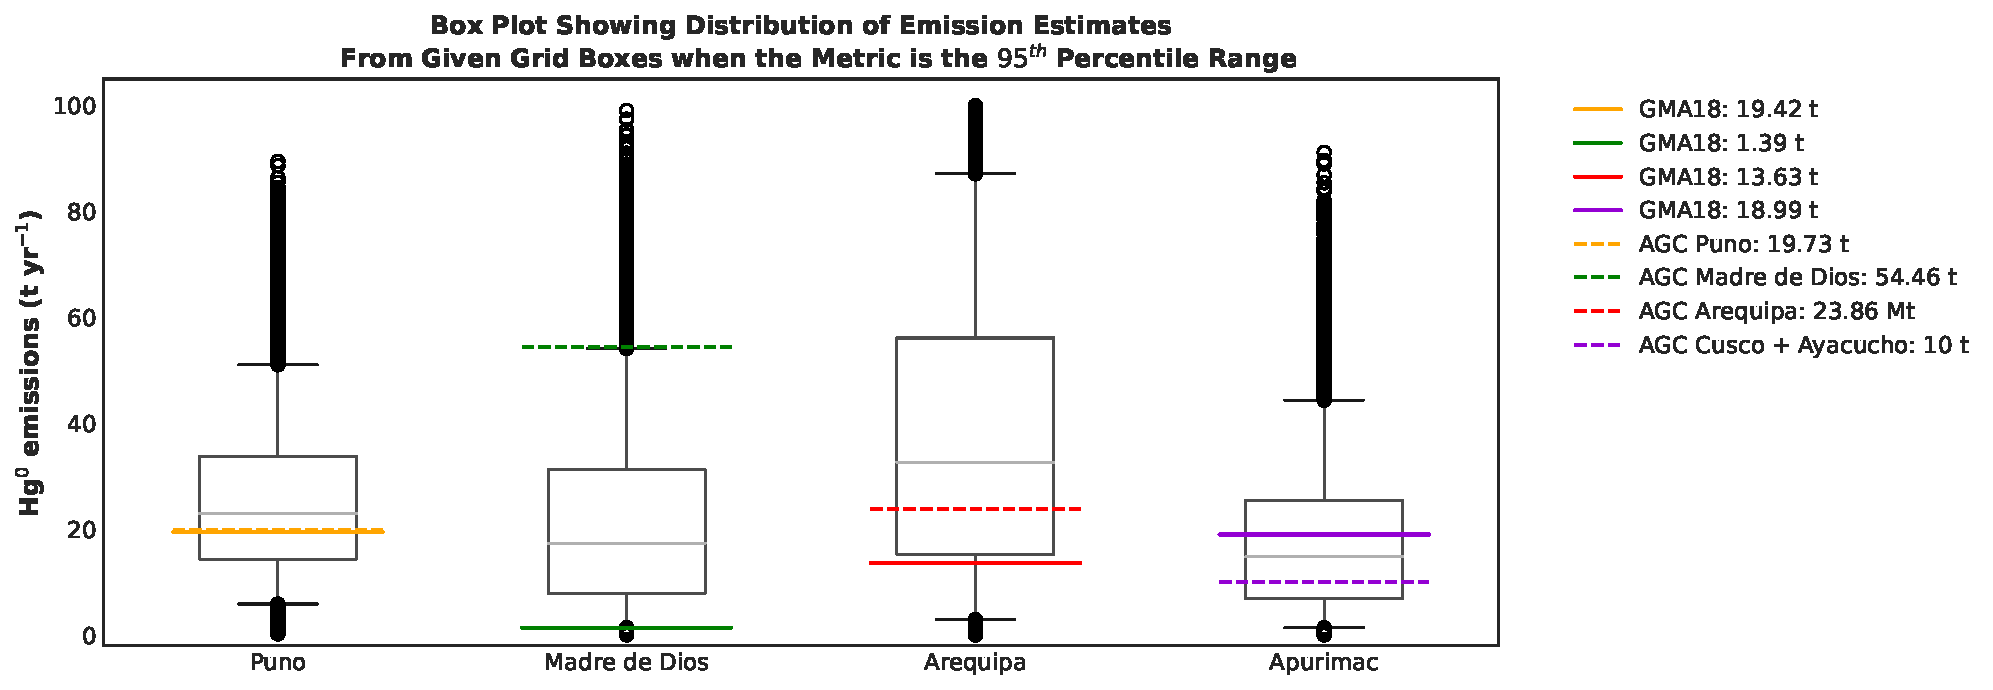
\includegraphics[width=\textwidth]{templates/figures/MCMC/MCMCMCMC_Estimates95th.pdf}
  \centering
  \caption{Emission Estimates when the $95^{th}$ percentile range is used as the metric to compare the model outputs to observations. The horizontal lines representing the emission estimates from the bottom-up inventories are traced over the box plots. The solid horizontal lines represent the emission estimates from the GMA 2018 inventory \cite{united_nations_environment_programme_technical_2019,steenhuisen_development_2019} and the dashed lines represent the emission estimates from the bottom-up inventory published by the Artisanal Gold Counsel\cite{agc_reporte_2017}.}
  \label{fig:MCMC_estimatesiqr}
\end{figure}
\FloatBarrier

\begin{figure}[H]
  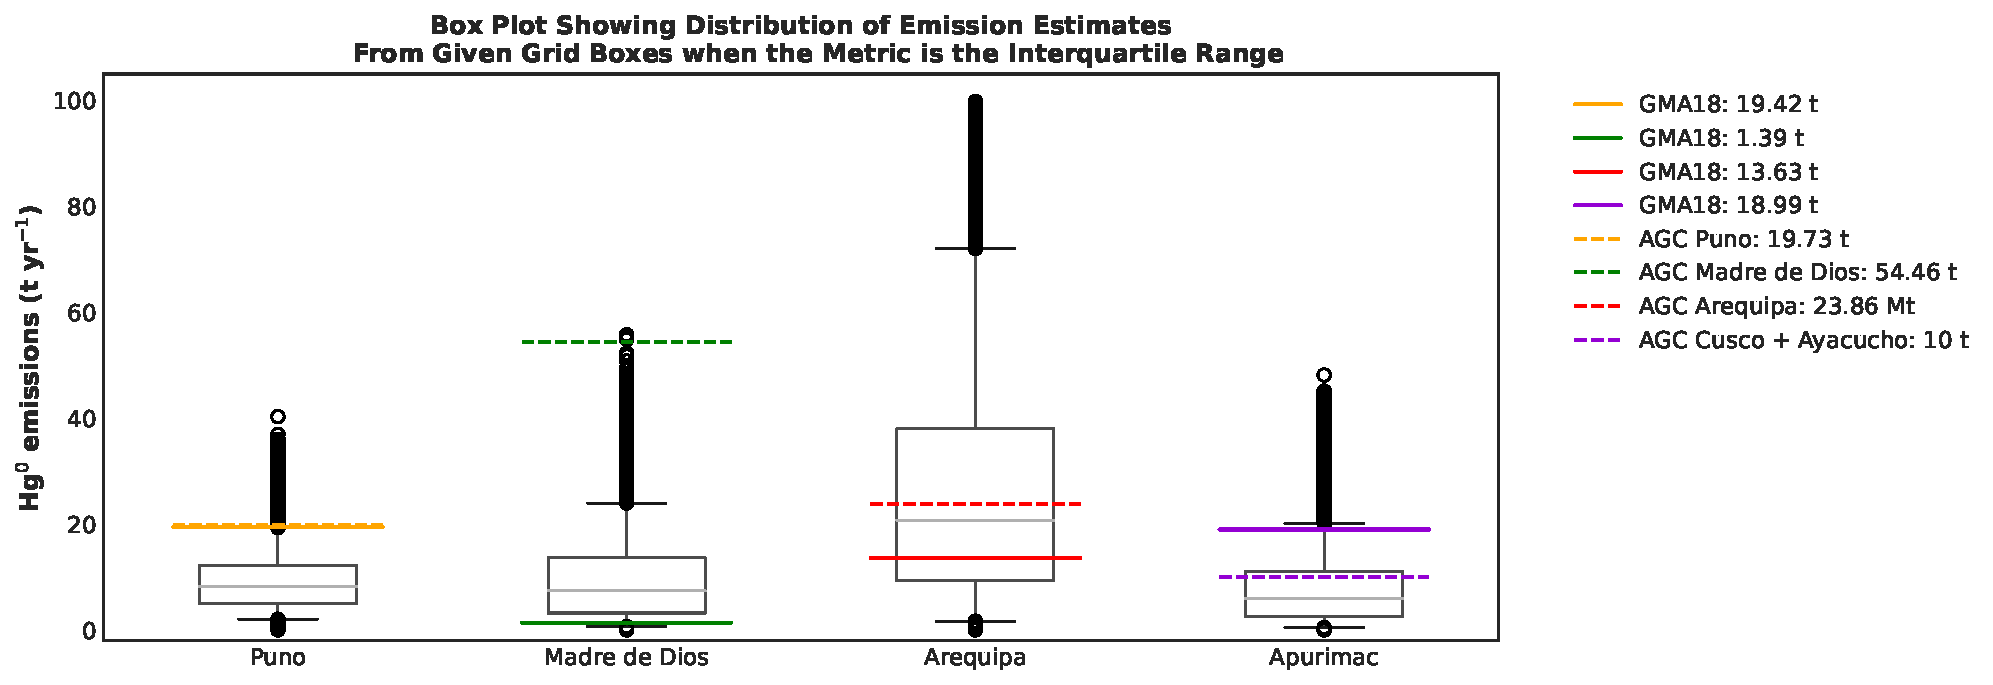
\includegraphics[width=\textwidth]{templates/figures/MCMC/MCMCMCMC_Estimatesiqr.pdf}
  \centering
  \caption{Emission Estimates when the IQR is used as the metric to compare the model outputs to observations. The horizontal lines representing the emission estimates from the bottom-up inventories are traced over the box plots. The solid horizontal lines represent the emission estimates from the GMA 2018 inventory \cite{united_nations_environment_programme_technical_2019,steenhuisen_development_2019} and the dashed lines represent the emission estimates from the bottom-up inventory published by the Artisanal Gold Counsel\cite{agc_reporte_2017}.}
  \label{fig:MCMC_estimates95}
\end{figure}
\FloatBarrier
\begin{flushleft}

\end{flushleft}

\section{Conclusion}